\documentclass[a4paper,12pt]{article}
\usepackage[utf8]{inputenc}
\usepackage{graphicx}
\graphicspath{ {img/} }
\usepackage[section]{placeins}

\setlength{\oddsidemargin}{0mm}
\setlength{\evensidemargin}{-14mm}
\setlength{\marginparwidth}{0cm}
\setlength{\marginparsep}{0cm}
\setlength{\topmargin}{2mm}
\setlength{\headheight}{0mm}
\setlength{\headsep}{0cm}
\setlength{\textheight}{240mm}
\setlength{\textwidth}{168mm}
\setlength{\topskip}{0mm}
\setlength{\footskip}{10mm}
\setlength{\parindent}{8ex}

\begin{document}
	\begin{titlepage}
    		\begin{center}
        		\vspace*{1cm}
        
        		\textbf{ENEL403  State-space design for an inverted pendulum and 3 cart controller}
        
        		\vspace{0.5cm}
        		Lab Report
        
        		\vspace{1.5cm}
        
        		\textbf{Jono Kapene \\ 53044694}
        
        		\vfill
        		
\includegraphics[scale=0.6]{pmeme.jpg}
        		\vspace{0.8cm}
        
        		Group E16\\
        		University of Canterbury\\
        		15th May, 2017
        
    \end{center}
\end{titlepage}
	\clearpage
	
\section{Abstract}
The aim of this lab was to design a state space controller for an inverted pendulum and a triple cart. The controller designs were first simulated in MatLab before they were tested in the lab. Two controllers were designed for both system, one using LQR method, which is detailed in the method section of this report, and manually placing the poles ourselves. Both systems had a set of specification, detailed in the introduction section of this report, and a set of possible parameter, such as mass and length. The controller designs should have been robust enough to work with all configurations in the lab.\\
The inverted pendulum design worked in matlab but failed when tested in the lab. Possible explanations for this are disscussed in the discussion section of this report. The LQR triple cart design worked much better than the manully placed pole design but could be imporved on with more work.

\section{Introduction}

This report details the state space design for a inverted pendulum controller, and a triple cart controller. These controller design were first modelled and simulated in the program MatLab and then tested on the actual thing. Two controllers were designed, one using LQR method and the other and manually placing poles.The inverted pendulum was modeled using the given state space equation in the form $$\dot{X}=AX+B_1U,Y=C_1X$$.

\begin{center}
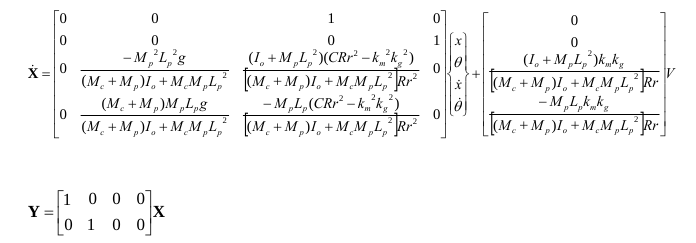
\includegraphics[scale=0.4]{iP_matrix.png}
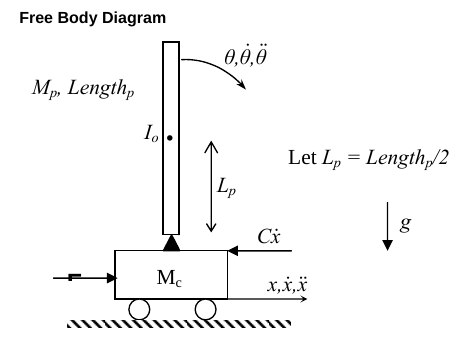
\includegraphics[scale=0.3]{iP_diagram.png}\\
\end{center}
\noindent
The design criteria for the inverted pendulum was as follows
\begin{enumerate}
\item setting time for $x$ and $\theta$ of $t_s < 5-7 seconds$
\item Rise time for $x$ and $\theta$ of $t_r < 1-3 seconds$
\item Overshoot of $\theta$ $M_p < 10$
\item Steady-state error of $e_ss < 2$\%
\item The input to the system $V < 10V$
\item The input to the system $dV/dt < 30 V/s$
\end{enumerate}
\noindent
The triple cart system is modelled from the diagram below.
\begin{center}
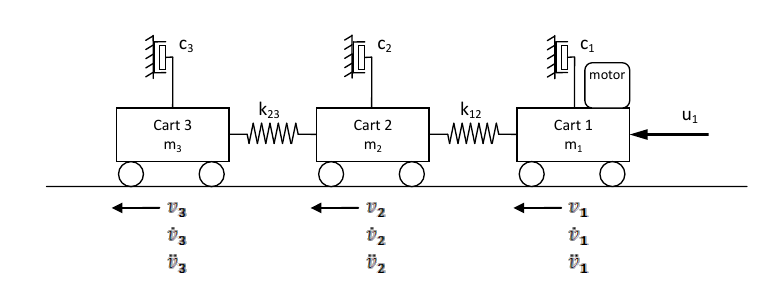
\includegraphics[scale=0.3]{3cart_diagram.png}\\
\end{center}
The 3 cart systemt controller's design constraints are as follows. The car must beable to accurately track 250mm and 500mm step inputs as quick as possible so the controller must be able to handle fast rise and settling times. The system needs to be robust enough as there is 12 possible combinations for the cart set up. Three different springs could be used as well as additional weights can be added to cart 2 and 3. The controller effort cannot surpass $\pm12V$ as this is the maximum the motor can take.

\section{Method}

\indent
The systems were modeled in matlab using $ss()$ function. To confirm that the systems are currently unstable, the poles of matrix A are found by using the $eig(A)$ function in MatLab. All poles must be negative to be stable. To stabilize the system, feedback was introduced. For this to be possible all four states must be controllable, which was found by using the $ctrb()$ and $rank()$ functions.\\

After the system has been verified unstable and fully controllable, the controller can now be designed. The first method used was linear quadratic regulation to determine the state feedback control gain matrix $K$. The matlab function lqr was used which parameters change the relative importance of the controller effort and error. The simpilist Q and R are chosen to find the first set of gains : $$Q = C'*C$$ $$R = 1$$ $$K = lqr(A,B1,Q,R)$$

Creating the state space equations for the new closed loop system:
$$Ac = [(A-B*K)];$$;
$$B1c = [B1];$$
$$C1c = [C1];$$
$$Dc = [D];$$

By increasing the values in the Q matrix you can increase the weight the controller has on the errors at the cost of increased controller effort. The Q matrix was changed by trial and error to meet the specifications.
Once the controller has met the rest of our specifications, precompenstion(N) needs to be added to meet our steady state error requirements. Firstly the C matrix is modified so only $x$ (Cart position) is affected as there is no steady state error from $\theta$.$$CN = [1 0 0 0]$$ $$sys_ss = ss(A,B1,CN,D)$$ $$N = rscale(sys_ss,K)$$

To manually place the poles the Matlab function $place()$ was used. The poles were determined using pole diagrams and moving the poles to suit our constraints such as overshoot and settling time These state space models are a simulation of the lab models and appropriate graphs are plotted below in the \emph{results} section of this report.\\

\section{Results}
\begin{figure}[h]
\centering
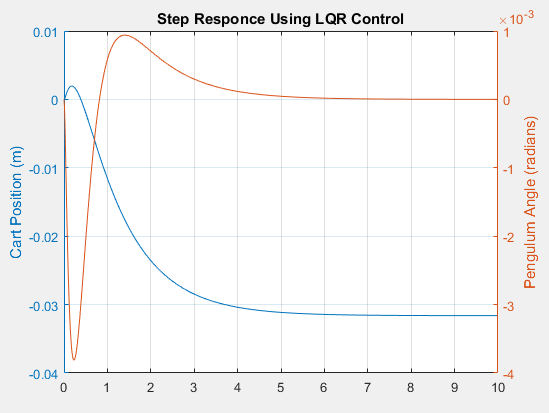
\includegraphics[scale=0.4]{iP_figure1.png}
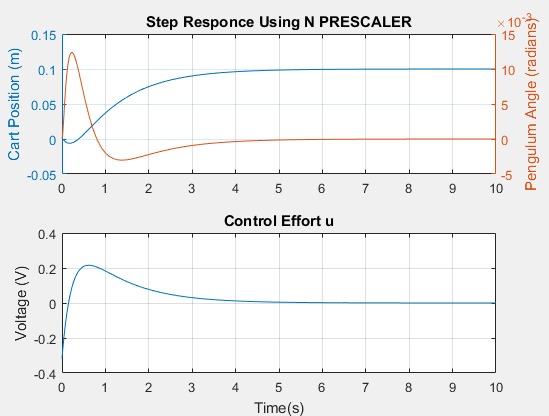
\includegraphics[scale=0.4]{iP_figure2.png}
\caption{Simulated inverted pendulum with and without precompensation}
\end{figure}

\begin{figure}[h]
\centering
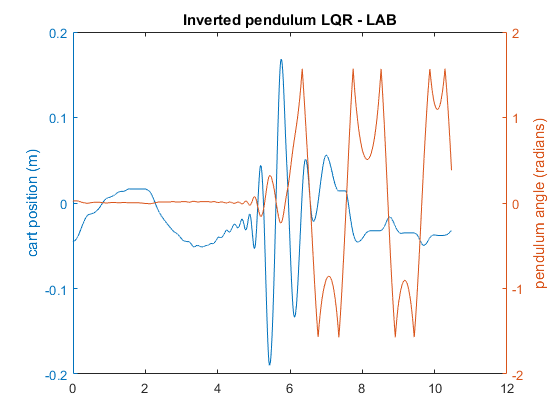
\includegraphics[scale=0.4]{lqrip-lab.png}
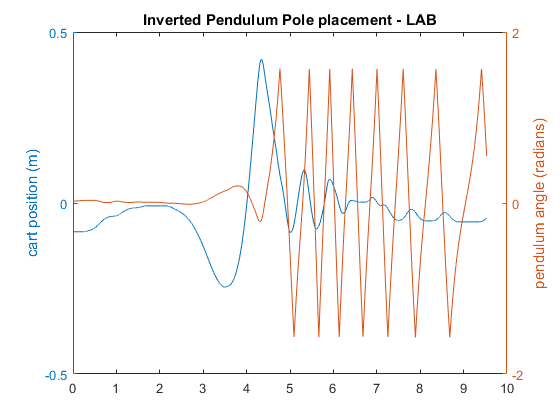
\includegraphics[scale=0.4]{ppip-lab.png}
\caption{Lab results for the inverted pendulum.}
\end{figure}

\begin{figure}[h]
\centering
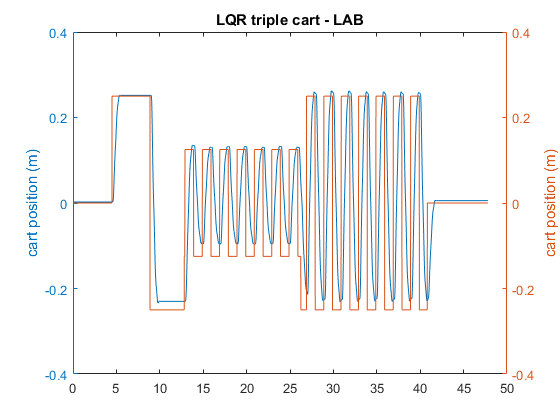
\includegraphics[scale=0.4]{lqr3cart-lab.png}
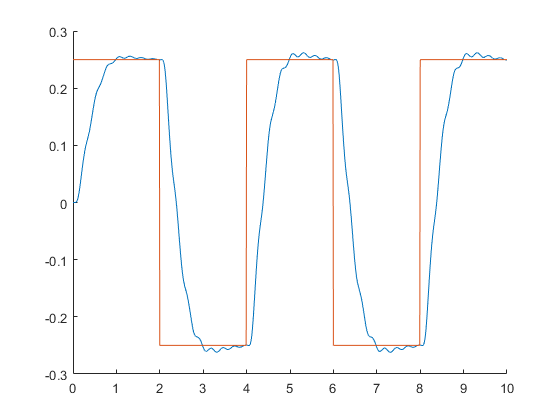
\includegraphics[scale=0.4]{lqr3cart-sim.png}
\caption{Lab and simulated data for the triple cart LQR controller.}
\end{figure}

\begin{figure}[h]
\centering
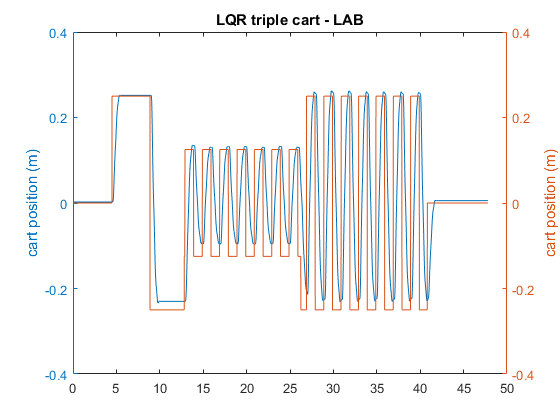
\includegraphics[scale=0.4]{lqr3cart-lab.png}
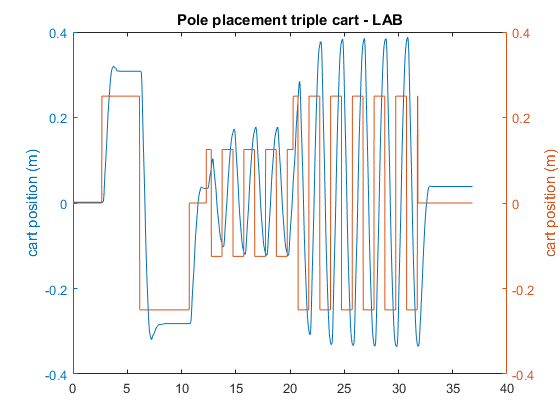
\includegraphics[scale=0.4]{pp3cart-lab.png}
\caption{Lab results for the triple cart.}
\end{figure}

\section{Discussion}
Figure 1 shows that the LQR gains work in our simulated enviroment and fit most of the specifications required however the cart has a steady state error which is improved by adding the prescaler. It goes from -0.03 to 0.1 as the step input is 0.1. So now when the cart is moved 10cm the controller controls the pendulums angle back to 0 degrees. The right graph shows how the low values in the Q matrix mean the controller effort is minimal. This system could be improved even more if the Q matrix was increased however the system meets the specifications and so the least controller effort the better.\\

Figure 2 shows the LQR and manually placed pole systems in the lab.  Both systems failed even though the simulations in matlab show different. We believe the system simulated was not robust enough and the pendulum in the lab was not the values that we expected. Another reason could have been that the prescaler in the simulation and the lab was different. When looking back at the lab data we can see that the tracking gain entered for both was 20, which cannot be correct as N depends on K and the lqr and poleplacement systems had different K vectors.\\

Figure 3 shows the lqr control system for the triple cart. The simulation shows a 0.25m pulse train input and the system follows the commands nicely.The Q matrix for this system was set so most of the controllers effort would be on cart 3 as thats the one that was moving the others. The exact values of Q were found by trial and error, checking it met the specifications and the controller effort did not exceed 10V. There is a noticable ripple where the carts settle that is not noticable in the real world lab. The ripple disappears due to the friction of the carts in the real world, which acts as a damper to smooth out those edges. The system works well as it has a small overshoot and little steady state error. The system does not appear to settle when t becomes small. It would be better if we had tested this system with a slighty longer pulse width to see how the system would have settled. The graph also shows that the higher values of cart postion have less error than the lower ones. At one end of the track the cart was heavier than the other due to the carts electrical cables (Assuming for the motor or sensors). This would cause the mass of the cart to change depending on the position of the cart. \\

Figure 4 shows the difference between the LQR design and the pole placements. The pole placements design has a much more noticable overshoot and steady state error. This is most likely from our poles not being robust enough for all the different combination of the cart and the uncertainty in the carts parameters given.


\section{Conclusion}
The aim of this lab was to design a state space controller for an inverted pendulum and a triple cart system. The inverted pendulum design was working in a matlab simulation but did not work in the lab. We think it didn't work because our design was not robust enough for all the configurations of the pendulum and our tracking gain was not correctly determined. The lqr triple cart design met the given specififcation and performed better than our pole placement design but there could have been some improvements such as increasing the pulse train width slightly.

\end{document}